\section{Definire cos'\`e un dipolo elettrico e calcolare il campo
	elettrico sull'asse del dipolo ed il potenziale che questo
	produce.}
Un \textbf{Dipolo elettrico} \`e un sistema composto da due cariche elettriche $+q$ e $-q$ poste a una distanza $d$, costante nel tempo.

\begin{center}
	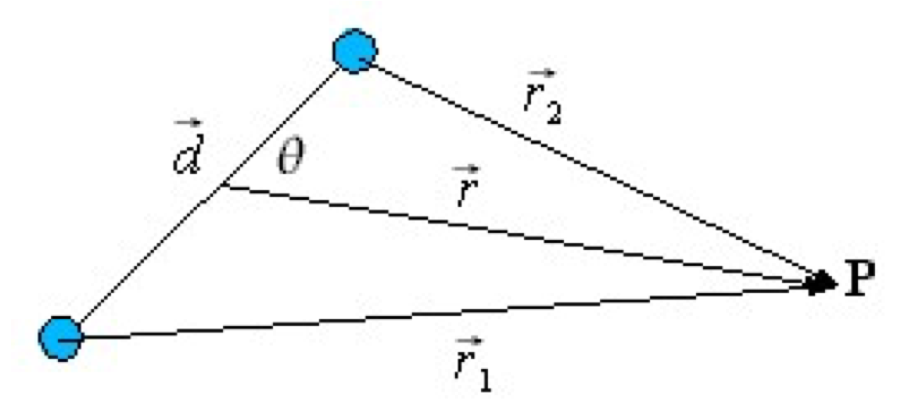
\includegraphics{dipolo} \\
	\textbf{Esempio grafico :} in un dipolo elettrico \`e interessante calcolare campo elettrico o potenziale di un dipolo in un punto generico $P$.
\end{center}

Si definisce \textbf{momento di dipolo} il seguente valore : 
\begin{equation}
    \vec{p} = q\vec{d}
\end{equation}

\textbf{Esempio 1 :} calcolo del campo elettrico lungo l'asse del dipolo.\\

Per comodit\'a si considera un dipolo di due cariche $q_1$ e $q_2$ situate nei punti A(+a, 0) e B(-a, 0), da cui ne ricaviamo il punto medio nell'origine del sistema di assi cartesiani di riferimento.\\
\\
Sapendo che il campo elettrico ha la seguente definizione
\begin{equation}
	\vec{E}(\vec{r}) = \frac{1}{4 \pi \varepsilon_0} \frac{q}{r^2} \hat{r}
\end{equation}
e per il \textbf{Principio di Sovrapposizione} sappiamo che
\begin{equation}
    \vec{E}(\vec{r}) = \sum_{j = 0}^{n_{cariche}}{\vec{E}_i(\vec{r})}
\end{equation}
Pertanto per il dipolo in questione il \textbf{Campo Elettrico} si definisce $\vec{r} = a\hat{i} + d\hat{j}$, dove $d (= 0)$ \`e la distanza del punto dall'asse del dipolo.
$$ \vec{E}(\vec{r}) = \frac{1}{4 \pi \varepsilon_0} \left(\frac{q}{(r_x - a)^2} - \frac{q}{(r_x + a)^2}\right)\hat{i} =
$$
$$ \frac{1}{4 \pi \varepsilon_0} \left(\frac{q}{(r_x - a)^2} - \frac{q}{(r_x + a)^2}\right)\hat{i} = 
$$
$$
\frac{1}{4 \pi \varepsilon_0} \left(\frac{q(r_x + a)^2 - q(r_x - a)^2}{(r_x^2 - a^2)^2}\right)\hat{i} = 
$$
$$
\frac{1}{4 \pi \varepsilon_0} \left(\frac{q\left[(r_x + a)^2 - (r_x - a)^2\right]}{(r_x^2 - a^2)^2}\right)\hat{i}
$$
Usando il metodo della \textbf{differenza dei quadrati} $\left[a^2 - b^2 = (a+b)(a-b)\right]$:
$$
\frac{1}{4 \pi \varepsilon_0} \left(\frac{q\left[(2r_x)(2a)\right]}{(r_x^2 - a^2)^2}\right)\hat{i} = 
$$
$$
\frac{1}{4 \pi \varepsilon_0} \left(\frac{4qar_x}{(r_x^2 - a^2)^2}\right)\hat{i}
$$
imponendo $2a = d$ (poich\`e $+a$ e $-a$ rappresentano dove si trovano le cariche sull'asse e la loro distanza \`e appunto $2a$):
$$
\frac{1}{4 \pi \varepsilon_0} \left(\frac{2qdr_x}{\left[r_x^2 - \left(\frac{d}{2}\right)^2\right]^2}\right)\hat{i}
$$
in termini del \textbf{momento di dipolo} dato da (8):
$$
\frac{1}{4 \pi \varepsilon_0} \left(\frac{2pr_x}{\left[r_x^2 - \left(\frac{d}{2}\right)^2\right]^2}\right)\hat{i}
$$
Ipotizzando che $r_x >> d$ si ottiene:
$$
\frac{ 1 }{ 4 \pi \varepsilon_0 } 
\frac{ 2pr_x }{ (r_x^2)^2 } 
\hat{ i } = 
\frac{ 1 }{ 4 \pi \varepsilon_0 } 
\frac{ 2p\cancel{ r_x } }{ r_x^{\cancel{ 4 }^3} } 
\hat{ i } = 
\frac{ 1 }{ 4 \pi \varepsilon_0 } 
\frac{ 2p}{ r_x^3 } 
\hat{ i }
$$
$\hfill\square$ \\
\textbf{Esempio 2 :} Calcolo del \textbf{potenziale elettrico} del dipolo sull'asse del dipolo.\\
Si ricorda la formula del potenziale elettrico come:
$$
  V(r_x) = \frac{1}{4 \pi \varepsilon_0}\frac{q}{r}
$$ 
Anche qui vale il \textbf{Principio di Sovrapposizione}:
$$
  V(r) = \sum_{k = 0}^{n_{cariche}}{V_i(r)}
$$
Si fanno le stesse premesse dell'esempio 1.\\
$$ V(r_x) = \frac{1}{4 \pi \varepsilon_0} \left(\frac{q}{r_x - a} - \frac{q}{r_x + a}\right) =
$$
$$
\frac{1}{4 \pi \varepsilon_0} \left(\frac{q(r_x + a) - q(r_x - a)}{r_x^2 - a^2}\right) = 
$$
$$
\frac{ 1 }{ 4 \pi \varepsilon_0 } \left( \frac{ q \left[ \cancel{ r_x } + a - \cancel{ r_x } + a \right] }{ r_x^2 - a^2 } \right) =
$$
$$
\frac{1}{4 \pi \varepsilon_0} \left(\frac{2aq}{r_x^2 - a^2}\right) =
$$
imponendo $2a = d$
$$
\frac{ 1 }{ 4 \pi \varepsilon_0 } 
\left( 
    \frac{ dq }{ r_x^2 - 
	\left( 
        \frac{ d }{ 2 } 
    \right) ^2 
    } 
\right) =
$$
in termini del \textbf{momento di dipolo} dato da (8):
$$
\frac{1}{4 \pi \varepsilon_0} \left(\frac{p}{r_x^2 - \left(\frac{d}{2}\right)^2}\right)
$$
Ipotizzando che $r_x >> d$ si ottiene:
$$
\frac{1}{4 \pi \varepsilon_0} \left(\frac{p}{r_x^2}\right) = \frac{ p }{ 4 \pi \varepsilon_0 r_x^2}
$$
$\hfill\square$ \\